\documentclass[11pt]{article}

\usepackage[utf8]{inputenc}
\usepackage[spanish, es-tabla]{babel}
\usepackage{mathtools}
\usepackage{amssymb}
\usepackage{amsthm} 
\usepackage{graphicx}
\usepackage{dsfont}

%Gummi|065|=)
\title{\textbf{Ejemplos}}
\author{Pedro Bonilla Nadal\\
		Johanna Capote Robayna\\
		Guillermo Galindo Ortuño}
\date{}

%No indent
\setlength\parindent{0pt}
\begin{document}

\maketitle
\section*{Programa 1} 
\underline{Datos} 
\begin{itemize}

\item $a = 0, b=1$
\item $ n = 10$
\item $k = 3 $
\item $f(t,y) = -y + t +1$ 

\end{itemize}

\underline{Solución} \\
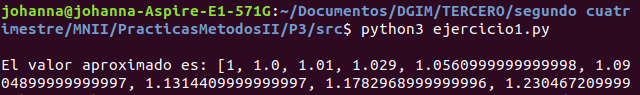
\includegraphics[width=1.1\textwidth]{../img/ej1} \\
\section*{Programa 3}
\underline{Datos}
\begin{itemize}
 
\item $a = 0, b=1$
\item $ n = 5$
\item $k = 3$
\item $ y0 = 1$
\item $f = -y+t+1$
\end{itemize}

\underline{Solución} \\
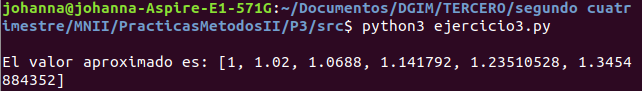
\includegraphics[width=1.1\textwidth]{../img/ej3}


\section*{Programa 5}
\underline{Datos}
\begin{itemize}

\item $a = 0, b=1$
\item $ n = 5$
\item $ k = 3$
\item $f = -y+t+1$ 
\end{itemize}

\underline{Solución} \\
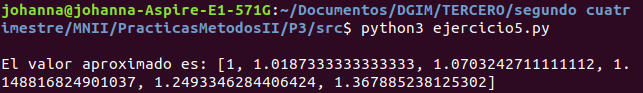
\includegraphics[width=1.1\textwidth]{../img/ej5} \\

\section*{Programa 9}
\underline{Datos}
\begin{itemize}

\item $a = 0, b=1$
\item $ n = 10$
\item $ k = 3$
\item $f = -y+t+1$ 
\end{itemize}

\underline{Solución} \\
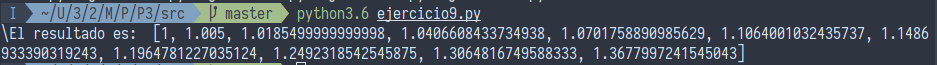
\includegraphics[width=1.1\textwidth]{../img/ej9} \\





\end{document}
